\documentclass[11pt]{article}

% --- packages (all present in a standard TeX Live / arXiv toolchain) ---------
\usepackage[utf8]{inputenc}
\usepackage[T1]{fontenc}
\usepackage{lmodern}
\usepackage[margin=1in]{geometry}
\usepackage{microtype}
\usepackage{amsmath}
\usepackage{booktabs}
\usepackage{graphicx}
\usepackage{xcolor}
\usepackage{listings}
\usepackage{pgfplots}
\pgfplotsset{compat=1.17}
\usepackage[numbers,sort&compress]{natbib}
\usepackage[colorlinks=true,linkcolor=black,citecolor=blue,urlcolor=blue]{hyperref}

% --- generated numbers: single source of truth (paper/make_results.py) -------
% AUTO-GENERATED by paper/make_results.py -- do not edit by hand.
\newcommand{\numTools}{148}
\newcommand{\numServers}{20}
\newcommand{\numCategories}{91}
\newcommand{\numQueries}{41}
\newcommand{\metaToolTokens}{305}
\newcommand{\tokenizerName}{tiktoken cl100k\_base}
\newcommand{\flatAccOne}{92.7}
\newcommand{\graphAccOne}{97.6}
\newcommand{\flatAccK}{100.0}
\newcommand{\graphAccK}{100.0}
\newcommand{\flatMRR}{0.963}
\newcommand{\graphMRR}{0.988}
\newcommand{\flatColl}{95.1}
\newcommand{\graphColl}{100.0}
\newcommand{\avgTok}{531}
\newcommand{\rawTokFull}{9041}
\newcommand{\reductionFull}{94.1}
\newcommand{\kval}{5}
\newcommand{\reductionSeventyFive}{88.6}
% corpus/query structure + shipped retriever hyperparameters
\newcommand{\numSingletonCategories}{60}
\newcommand{\medianCategorySize}{1}
\newcommand{\maxCategorySize}{6}
\newcommand{\numLinkedConcepts}{88}
\newcommand{\numAltEdges}{204}
\newcommand{\numOtherEdges}{0}
\newcommand{\numDistractors}{71}
\newcommand{\numCrossServerDistractors}{61}
\newcommand{\numResolvableDistractors}{70}
\newcommand{\numCasesWithDistractor}{41}
\newcommand{\denseDim}{256}
\newcommand{\ngramSizes}{3,4,5}
\newcommand{\ngramWeight}{0.5}
\newcommand{\bmWeight}{0.5}
\newcommand{\denseWeight}{0.5}
\newcommand{\bmKOne}{1.5}
\newcommand{\bmB}{0.75}
\newcommand{\hierBoost}{0.15}
\newcommand{\hierTopCats}{2}
\newcommand{\graphMaxPerHit}{3}
\newcommand{\maxAlternatives}{5}
\newcommand{\altDamping}{0.85}
\newcommand{\otherDamping}{0.6}
\newcommand{\denseAccOne}{92.7}
\newcommand{\denseColl}{100.0}
\newcommand{\hybridBareAccOne}{97.6}
\newcommand{\hybridBareColl}{100.0}
\newcommand{\bmHierAccOne}{92.7}
\newcommand{\bmGraphAccOne}{92.7}


% --- listing style for OKT markdown ------------------------------------------
\definecolor{kw}{RGB}{30,70,200}
\definecolor{cm}{RGB}{110,120,135}
\definecolor{str}{RGB}{20,130,70}
\lstdefinestyle{okt}{
  basicstyle=\ttfamily\small,
  keywordstyle=\color{kw},
  commentstyle=\color{cm}\itshape,
  stringstyle=\color{str},
  showstringspaces=false,
  breaklines=true,
  frame=single,
  rulecolor=\color{black!20},
  columns=fullflexible,
}

\title{\textbf{OKTS: Open Knowledge Tool Search\\
(Progressive Tool Disclosure with Portable Descriptors)}}
\author{PrabhuKiran Ganapavarapu\\
\small Independent Researcher \\
\small \texttt{prabhukiran.g@gmail.com} \\
\small ORCID: \href{https://orcid.org/0009-0001-9971-9589}{0009-0001-9971-9589}}
\date{\today}

\begin{document}
\maketitle

\begin{abstract}
Large language model (LLM) agents are increasingly given access to hundreds of
tools drawn from many sources (Model Context Protocol servers, plain functions,
HTTP/OpenAPI endpoints, sub-agents). Loading every tool's JSON schema into the
context window up front is the dominant pattern, but its cost scales with the
size of the catalog rather than the difficulty of the task, and is re-paid on
every turn: schemas consume a large fraction of the window before the task
begins, and near-duplicate tools across sources (\texttt{github.create\_issue} vs.\
\texttt{gitlab.create\_issue} vs.\ \texttt{linear.create\_issue}) blur together
and induce wrong selections. The common alternative---retrieval-augmented
generation (RAG) over tool embeddings---removes the up-front cost but replaces it
with standing \emph{infrastructure}: an embedding model to host or an API to
call, a vector store to maintain, and a re-embedding step on every catalog
change. We present \textbf{OKTS}, a source-agnostic runtime that (i) describes
each tool as a portable, git-versioned Markdown descriptor (the \textbf{OKT}
format) and (ii) serves any catalog behind a fixed three-tool interface
(\texttt{search\_tools}, \texttt{load\_tool}, \texttt{call\_tool}) via
\emph{progressive disclosure}. On a corpus of \numTools{} tools adapted from
\numServers{} widely used MCP servers, OKTS reduces per-query tool-schema tokens
by \textbf{\reductionFull\%} relative to the load-everything baseline, a
reduction that grows with corpus size. For ranking, OKTS uses a fully offline,
\emph{zero-infrastructure} hybrid retriever---BM25 combined with a deterministic
feature-hashing embedding that needs no model, API, or vector store---which lifts
top-1 tool-selection accuracy from \flatAccOne\% to \graphAccOne\% and eliminates
near-duplicate collisions (\flatColl\%~$\rightarrow$~\graphColl\%) over a strong
BM25 baseline, at essentially identical token cost. An ablation is reported
faithfully: the gain comes from \emph{fusing} the two lexical signals---neither
BM25 nor the hashing embedding reaches it alone---and not from the
category-hierarchy prefilter or graph expansion, which are accuracy-neutral on
this corpus and instead serve to keep the returned-result count fixed and to
surface alternatives. All numbers are produced by a reproducible harness over an
open corpus.
\end{abstract}

% =============================================================================
\section{Introduction}
% =============================================================================

The prevailing way to give an LLM agent a tool is to place that tool's name,
description, and full JSON input schema into the model's context as a
function-calling definition. This works for a handful of tools and fails at
scale for two independent reasons.

\paragraph{Context cost.} Every tool definition is paid for in tokens on every
turn, whether or not the tool is used. With the standardization of the Model
Context Protocol (MCP)~\citep{mcp}, it is now routine for an agent to be wired to
many servers at once, each exposing tens of tools; the combined schemas can
consume a large fraction of the context window before the task begins, starving
the prompt and diluting attention across definitions the agent will never
call~\citep{liu2023lost}.

\paragraph{Selection cost.} As the catalog grows, it accumulates
\emph{near-duplicate} tools---especially across sources that wrap the same
capability. A query like ``open a bug ticket in my GitHub repo'' must select
\texttt{github.create\_issue} over the lexically almost-identical
\texttt{gitlab.create\_issue} and \texttt{linear.create\_issue}. Flat lexical
matching frequently picks the wrong sibling or hallucinates parameters.

The community response has largely been \emph{retrieval over tools}: index tool
descriptions, retrieve the top-$k$ for each query, and expose only those. When
the index is a dense vector store, this is RAG applied to
tools~\citep{patil2023gorilla,qin2023toolllm}. It solves the context-cost
problem but introduces a standing \emph{operational} cost that is easy to
overlook: a semantic index requires an embedding model (hosted locally or behind
an API), a vector store to persist and query, and a re-embedding pass whenever a
tool is added, edited, or removed. For a tool catalog---which changes far more
often than a document corpus and is small enough that heavyweight retrieval
infrastructure is disproportionate---this is a poor trade.

\paragraph{Contributions.} We describe \textbf{OKTS} (Open Knowledge Tool
Search), a runtime that keeps the benefit of retrieval while removing both the
up-front context cost \emph{and} the embedding infrastructure:

\begin{enumerate}
  \item \textbf{The OKT descriptor} (\S\ref{sec:okt}): a portable, human-readable,
    git-versioned Markdown file per tool, whose YAML frontmatter is grouped by the
    runtime phase that consumes it. It is the durable artifact a semantic index
    lacks---diffable, editable, and reviewable.
  \item \textbf{Progressive disclosure} (\S\ref{sec:method}): a fixed three-tool
    interface (\texttt{search\_tools}/\texttt{load\_tool}/\texttt{call\_tool})
    that returns lightweight refs, loads exactly one schema on demand, and
    dispatches the call---so tool-schema context is bounded and, empirically,
    near-constant regardless of catalog size (\reductionFull\% reduction at
    \numTools{} tools, growing with the corpus).
  \item \textbf{Zero-infrastructure hybrid retrieval} (\S\ref{sec:method},
    \S\ref{sec:results}): BM25 fused with a \emph{deterministic feature-hashing
    embedding}~\citep{weinberger2009hashing} that needs no model, no API, and no
    vector store, yet improves top-1 selection accuracy and eliminates
    near-duplicate collisions versus a strong BM25 baseline.
  \item \textbf{An honest empirical study} (\S\ref{sec:results}): a reproducible
    harness over an open \numTools-tool corpus, including an ablation that shows
    which structural signals help selection accuracy and which do not.
\end{enumerate}

A companion observation frames the comparison: swapping in a \emph{learned}
embedder is supported (an injectable \texttt{embed\_fn}) but would reintroduce
exactly the model/API/vector-store cost OKTS exists to avoid; we therefore
benchmark the zero-infrastructure default deliberately.

% =============================================================================
\section{Related Work}
% =============================================================================

\paragraph{Tool-using LLMs.} ReAct~\citep{yao2023react} and
Toolformer~\citep{schick2023toolformer} established interleaving reasoning with
tool calls. Scaling the number of tools motivated retrieval-based selection:
Gorilla~\citep{patil2023gorilla} retrieves API documentation, and
ToolLLM/ToolBench~\citep{qin2023toolllm} operate over thousands of real APIs with
a retriever front-end. These systems typically rank tools with a dense retriever,
inheriting the embedding-infrastructure cost discussed above.

\paragraph{Retrieval over tools to reduce prompt bloat.} The closest work
retrieves a small, relevant subset of tools per query instead of loading the
whole catalog. RAG-MCP~\citep{ragmcp} mitigates prompt bloat in LLM tool
selection by retrieving MCP tools with a retriever before invocation.
Toolshed~\citep{toolshed} scales tool-equipped agents through ``RAG-Tool
Fusion'' over a tool knowledge base. OKTS shares their retrieve-then-use premise
but differs on three axes: the retrieved unit is a \emph{portable, git-versioned
descriptor} (the OKT file) rather than an opaque vector; the runtime is
source-agnostic---MCP, functions, HTTP, sub-agents, and search---behind one
three-tool interface; and the default retriever needs \emph{no} embedding model,
API, or vector store, so adding or editing a tool never triggers a re-embedding
pass.

\paragraph{Retrieval.} Our ranker builds on BM25~\citep{robertson2009bm25} and,
for the hybrid variant, feature hashing (the ``hashing trick'')
\citep{weinberger2009hashing} as a deterministic, model-free embedding; score
fusion follows standard weighted-sum and reciprocal-rank-fusion
practice~\citep{cormack2009rrf}. Token counts use the \texttt{cl100k\_base} BPE
encoding~\citep{tiktoken}.

% =============================================================================
\section{The OKT Descriptor}
\label{sec:okt}
% =============================================================================

An \textbf{OKT} (Open Knowledge Tool) file is YAML frontmatter followed by a
Markdown body. The format is a \emph{profile} of the Open Knowledge Format
(OKF)~\citep{okf}, a portable Markdown-with-frontmatter convention for
representing organizational knowledge: OKT specializes it for a single callable
tool (\texttt{type:\,tool}). The frontmatter is emitted in groups, each labeled
with the runtime phase that consumes it, so an opened file is self-documenting
and a code review of a tool change is meaningful. Listing~\ref{lst:okt} is the
verbatim output of the runtime's serializer for one corpus tool.

\begin{lstlisting}[style=okt,caption={An OKT descriptor, exactly as the runtime serializes it. Frontmatter is grouped by consuming phase; the body is retrieval prose, never the calling contract. The \texttt{alternatives} edges were derived by the auto-linker, not declared by the source.},label={lst:okt}]
---
# identity
type: tool
id: github.search_issues
title: Search Issues

# match -- ranked by search_tools (phase 1); never sent at call time
description: Search issues and pull requests across repositories
  by free-text query.
tags:
- github
- mcp

# call -- loaded by load_tool (phase 2); the calling contract
input_schema:
  type: object
  required:
  - query
  properties:
    query:
      type: string

# route -- used by call_tool to dispatch (phase 3)
interface: mcp
target: github
side_effects: read
invocation: async

# graph edges -- expanded during search_tools
alternatives:
- github.create_issue
- github.get_issue
- github.list_issues
- github.update_issue
---

Synonyms: search, issues, github, mcp.

Use this to search issues and pull requests across repositories
by free-text query.

Gotcha: This is read-only and safe to call speculatively; it
does not modify state.
\end{lstlisting}

An optional \texttt{auth} field names a credential (e.g.\ \texttt{auth:
github\_token}); the runtime resolves it at dispatch through a pluggable secrets
provider---by default the environment variable \texttt{OKTS\_SECRET\_GITHUB\_TOKEN}
---so the value never appears in the descriptor or in agent context.

The format enforces five invariants. (1) The agent-facing surface is always
exactly three tools.\footnote{\texttt{call\_tool} additionally has an
\texttt{acall\_tool} coroutine form for awaiting asynchronous targets. It is the
same phase-3 tool under a different calling convention, not a fourth tool, and
hosts expose one or the other.} (2) \texttt{input\_schema} is always a structured
JSON Schema, so arguments can be validated before dispatch. (3) The body is
\emph{retrieval prose}, used only for ranking---never the calling contract.
(4) Credentials are resolved inside the runtime at dispatch and never enter agent
context. (5) A minimal descriptor requires only six fields
(\texttt{type}, \texttt{id}, \texttt{title}, \texttt{description},
\texttt{input\_schema}, \texttt{interface}); everything else is optional and
additive. A structural conformance check enforces exactly these rules before a
bundle is served---the six required fields present and non-empty, the
\texttt{type:\,tool} discriminator, \texttt{input\_schema} structured rather than
prose, \texttt{interface}/\texttt{side\_effects}/\texttt{invocation} drawn from
their known value sets, and every graph edge resolving to a concept in the same
bundle. We validate the OKT profile's own rules; we do not claim to validate
against a normative OKF schema, which is not published as a machine-checkable
artifact.

Descriptors are produced by adapters---one per source type
(\texttt{mcp}, \texttt{function}, \texttt{http}, \texttt{agent},
\texttt{search})---and then \emph{auto-linked}: a query-independent pass derives a
\texttt{server/resource} category hierarchy and \texttt{alternatives} edges
between near-duplicate tools from the flat set. The resource noun is the tool
name's last non-stopword \texttt{\_}-token, plural-stemmed
(\texttt{list\_issues}~$\rightarrow$~\texttt{issue}), and same-group members are
linked as mutual alternatives, capped at \maxAlternatives{} per tool for
determinism.

% =============================================================================
\section{Progressive Disclosure and Retrieval}
\label{sec:method}
% =============================================================================

\subsection{The three-tool interface and the token model}

Regardless of catalog size, the agent sees three tools:
\texttt{search\_tools(query, k)} returns up to $k$ lightweight refs
(id, title, description---\emph{no} schema); \texttt{load\_tool(id)} returns the
one structured \texttt{input\_schema} for the chosen tool; and
\texttt{call\_tool(id, args)} validates the arguments against that schema and
dispatches to the real source.

We account for tokens as an agent would pay them. Because function-calling APIs
re-send the tool definitions with every request, both quantities below are
per-query costs and are directly comparable. The \emph{baseline} loads all
$N$ tool schemas up front:
$C_\text{raw} = \sum_{i=1}^{N} \text{tok}(\text{schema}_i)$, where each
$\text{schema}_i$ is the tool's name, description, and JSON parameter schema
serialized as one function definition.
Under OKTS the per-query cost is
\begin{equation}
C_\text{OKTS} = \underbrace{C_\text{meta}}_{\text{3 tools} = \metaToolTokens} \;+\;
\sum_{j=1}^{k}\text{tok}(\text{ref}_j) \;+\; \text{tok}(\text{schema}_{\text{loaded}}),
\label{eq:cost}
\end{equation}
i.e.\ the constant three-meta-tool schemas, the $k$ lightweight refs, and the
\emph{single} schema loaded for the chosen tool. Crucially $C_\text{meta}$ and
the number of refs do not depend on $N$, so $C_\text{OKTS}$ is bounded as $N$
grows while $C_\text{raw}$ grows linearly. Token counts use
\tokenizerName{} (with a deterministic \texttt{chars/4} fallback when the encoder
is unavailable).

\subsection{Ranking: hybrid, then structure}

The baseline retriever is BM25~\citep{robertson2009bm25}
($k_1=\bmKOne$, $b=\bmB$) over each descriptor's match text---the concatenation
of \texttt{description}, \texttt{tags}, and body. The full retriever fuses BM25
with a dense score and then applies two structural steps.

\paragraph{Deterministic hashing-dense.} Rather than a learned embedder, the
default dense signal hashes features into a \denseDim-dimensional
L2-normalized vector via the hashing trick~\citep{weinberger2009hashing}: each
whitespace token and each character $n$-gram ($n \in \{\ngramSizes\}$, weighted
\ngramWeight{} relative to whole tokens) is mapped to a signed bucket by a SHA-1
digest, so the mapping is stable across processes and machines. Scoring is a dot
product, which equals cosine similarity on the normalized vectors. It is fully
deterministic, requires no model download or network call, and gives partial
credit for morphological variants (\texttt{issue}/\texttt{issues}) that a plain
BM25 tokenizer treats as unrelated. One asymmetry is deliberate: the dense side
embeds only a concept's \emph{own} \texttt{description} and \texttt{tags} and
excludes the body, so it describes what a tool \emph{is} rather than what it
mentions in passing. The motivating case is a hand-authored body that steers a
reader away from a sibling (``don't confuse this with \texttt{list\_issues}''),
which as raw text is lexically indistinguishable from an endorsement; BM25 keeps
the body, the dense signal does not. The two scores are
min-max normalized and combined by weighted sum with equal weights
($\bmWeight/\denseWeight$); reciprocal rank fusion is also
implemented~\citep{cormack2009rrf} and is not used in the reported
configuration. This is the entire ``embedding'' cost of OKTS: no model, no API,
no vector store, and nothing to re-embed when a tool changes.

\paragraph{Hierarchy prefilter and graph expansion.} Two optional structural
steps operate over the auto-linked bundle. The hierarchy prefilter scores each
category path by its stemmed token overlap with the query, normalized by path
length, and adds a flat $+\hierBoost$ to members of the top \hierTopCats{}
categories; nothing is ever removed (a harder \emph{restrict} mode exists but is
off by default), so this step cannot push the full retriever below the baseline.
Graph expansion pulls up to \graphMaxPerHit{} graph neighbors per top-ranked hit,
damped relative to their seed---$\times\altDamping$ across an
\texttt{alternatives} edge and $\times\otherDamping$ across
\texttt{composes\_with}/\texttt{prerequisites}. On this corpus the auto-linker
derives only \texttt{alternatives} edges, so only that damping is exercised.
Importantly, expansion is constrained to a \emph{fixed result count}: because
every sibling is damped strictly below its seed, siblings compete \emph{within}
the $k$ returned refs (the merged set is re-sorted and truncated to $k$) rather
than being appended past it. Consequently the top-1 result is always a rank hit,
and the returned-ref count---and hence the per-query token cost---stays fixed.
We emphasize that this is a \emph{result-count} constraint in code; the token
flatness in Eq.~\ref{eq:cost} is a measured consequence, not an enforced token
limit.

% =============================================================================
\section{Experimental Setup}
\label{sec:setup}
% =============================================================================

\paragraph{Corpus.} We assemble \numTools{} tools across \numServers{} widely
used MCP servers (GitHub, GitLab, Linear, Postgres, Supabase, BigQuery/GCP,
MongoDB, Redis, Qdrant, Docker, Kubernetes, AWS, Cloudflare, Vercel, Notion,
Figma, Sentry, Playwright, Chrome DevTools, filesystem). \emph{The tool lists are
hand-authored approximations of each server's published surface}---realistic
names and compact schemas with the cross-server near-duplicates that make
selection hard---not live captures; the ingestion path is identical to a live
capture (only the source of the \texttt{tools/list} payload differs).

Each \texttt{tools/list} payload passes through the ordinary offline build:
adapt~$\rightarrow$~enrich~$\rightarrow$~auto-link~$\rightarrow$~validate. We
stress that the enrichment step is a \emph{deterministic offline} enricher, not
an LLM: it emits a fixed template of synonyms drawn from the tool's own id and
tags, a restatement of the description, and a side-effect gotcha (visible in the
body of Listing~\ref{lst:okt}). The retrieval text is therefore mechanically
derived, which is the conservative setting---an LLM enrichment pass, which the
runtime also supports, would add genuine synonyms and would if anything raise
absolute accuracy.

The auto-linker derives \numCategories{} categories, of which
\numSingletonCategories{} contain a single tool (median category size
\medianCategorySize{}, maximum \maxCategorySize{}), and \numAltEdges{}
\texttt{alternatives} edges covering \numLinkedConcepts{} of the \numTools{}
tools. It derives no \texttt{composes\_with}/\texttt{prerequisites} edges from a
flat \texttt{tools/list}, so graph expansion here operates purely over
\texttt{alternatives}.

\paragraph{Queries.} A labeled set of \numQueries{} natural-language queries, each
mapping to one correct tool id plus a list of \texttt{distractors}: the
wrong-but-tempting near-duplicates the retriever must not prefer. There are
\numDistractors{} distractors in total (mean $1.7$ per query, and every query has
at least one), of which \numCrossServerDistractors{} name a tool on a
\emph{different} server than the correct answer---the cross-server collision
failure mode---and the remainder a sibling on the same server.

\paragraph{Metrics.} We report accuracy@1 and accuracy@$k$ (is the correct tool
ranked first / in the top $k$), mean reciprocal rank (MRR), and
\emph{collision-avoidance}: the fraction of queries in which the correct tool
outranks every one of its listed distractors that appears in the returned
set.\footnote{The implementation also counts a query as avoided when neither the
correct tool nor any distractor is returned at all, which would make the metric
vacuously satisfiable. That branch is never taken here: accuracy@$k$ is
\graphAccK\% for every configuration in Tables~\ref{tab:main}
and~\ref{tab:ablation}, so the correct tool is always present and every query is
scored against at least one distractor
(\numResolvableDistractors{}/\numDistractors{} distractor ids resolve to a tool
in the corpus).} We report token cost alongside every accuracy number, never one
without the other: the raw all-schemas cost, the average per-query OKTS cost
(Eq.~\ref{eq:cost}), and the reduction. We use $k=\kval$ throughout.

% =============================================================================
\section{Results}
\label{sec:results}
% =============================================================================

\subsection{Selection accuracy and token cost}

Table~\ref{tab:main} compares the flat BM25 baseline against the full retriever.
The full retriever raises accuracy@1 from \flatAccOne\% to \graphAccOne\%, raises
MRR from \flatMRR{} to \graphMRR{}, and eliminates near-duplicate collisions
(\flatColl\%~$\rightarrow$~\graphColl\%), at essentially identical per-query token
cost ($\approx\avgTok$ tokens). Both retrievers reach \flatAccK\%
and \graphAccK\%~accuracy@$k$ respectively: on this corpus the correct tool is
always \emph{within} the top $\kval$, so the differentiation is entirely at the
top rank and in collision avoidance. This also bounds how much a better ranker
could gain here---the headroom is a re-ordering problem, not a recall problem.

\begin{table}[h]
\centering
\caption{Flat BM25 baseline vs.\ the full OKTS retriever on \numTools{} tools,
\numQueries{} labeled queries, $k=\kval$. Token cost is per query.}
\label{tab:main}
% AUTO-GENERATED by paper/make_results.py
\begin{tabular}{lccccc}
\toprule
Retriever & acc@1 & acc@$k$ & MRR & coll.\ avoid. & avg tok/qry \\
\midrule
Flat BM25 (baseline) & 92.7 & 100.0 & 0.963 & 95.1 & 532 \\
\textbf{Graph-aware (ours)} & \textbf{97.6} & 100.0 & \textbf{0.988} & \textbf{100.0} & 531 \\
\bottomrule
\end{tabular}

\end{table}

\subsection{What actually drives the gain (ablation)}

Table~\ref{tab:ablation} isolates each signal. The result is reported as
measured, including where it is null. The accuracy gain comes \emph{entirely from
the hybrid (BM25 + hashing-dense) ranking}: ``Hybrid, no structure'' already
reaches \hybridBareAccOne\% accuracy@1 and \hybridBareColl\%
collision-avoidance---the full retriever's numbers exactly. Adding the hierarchy
prefilter or graph expansion on top does not further improve accuracy@1 or
collision-avoidance on this query set, and neither structural signal alone moves
the BM25 baseline (\bmHierAccOne\% and \bmGraphAccOne\% accuracy@1, versus
\flatAccOne\% for BM25 alone).

Three honest readings follow. First, the effect is one of \emph{complementarity},
not of either signal being stronger: BM25 alone and hashing-dense alone both sit
at \flatAccOne\%/\denseAccOne\% accuracy@1, and only their fusion reaches
\hybridBareAccOne\%. The dense signal does carry collision-avoidance on its own
(\denseColl\%), which is consistent with its intended role---giving morphological
partial credit that exact-token BM25 misses on near-duplicate names. Second, no
learned embedding is involved anywhere in this gain. Third, the hierarchy is far
too fine-grained on this corpus to discriminate: \numSingletonCategories{} of the
\numCategories{} derived categories contain exactly one tool (median size
\medianCategorySize{}), so boosting the top \hierTopCats{} categories most often
boosts the single tool that was already winning. Graph expansion, in turn, is
\emph{designed} not to alter the top rank, since siblings are damped strictly
below their seed. Their value is preserving the fixed return count while
surfacing alternatives---and, plausibly, scoping corpora larger or flatter than
this one---not lifting accuracy@1 on this set. We do not have evidence for the
larger-corpus claim and do not assert it.

\begin{table}[h]
\centering
\caption{Ablation. The accuracy gain is attributable to hybrid ranking; the
structural signals are accuracy-neutral here (see text).}
\label{tab:ablation}
% AUTO-GENERATED by paper/make_results.py
\begin{tabular}{lccccc}
\toprule
Configuration & acc@1 & acc@$k$ & MRR & coll.\ avoid. & avg tok/qry \\
\midrule
BM25 only (baseline) & 92.7 & 100.0 & 0.963 & 95.1 & 532 \\
Dense only (hashing) & 92.7 & 100.0 & 0.957 & 100.0 & 530 \\
Hybrid, no structure & 97.6 & 100.0 & 0.988 & 100.0 & 531 \\
BM25 + hierarchy & 92.7 & 100.0 & 0.963 & 95.1 & 532 \\
BM25 + graph & 92.7 & 100.0 & 0.963 & 95.1 & 530 \\
Hybrid + hierarchy + graph & 97.6 & 100.0 & 0.988 & 100.0 & 531 \\
\bottomrule
\end{tabular}

\end{table}

\subsection{Token reduction grows with the corpus}

Figure~\ref{fig:reduction} sweeps corpus size. Sub-corpora are prefixes of the
full bundle in its canonical (server-alphabetical) order, re-auto-linked at each
size, with the same \numQueries{} queries run against each; only the token
accounting is read off this sweep, never accuracy, since a truncated corpus does
not contain every query's answer. Because $C_\text{OKTS}$ is bounded
(Eq.~\ref{eq:cost}) while $C_\text{raw}$ grows linearly, the reduction climbs from
a modest fraction on a tiny corpus to \reductionFull\% at the full \numTools{}
tools (\reductionSeventyFive\% already at 75 tools), crossing 85\% at roughly 60
tools. The per-query OKTS cost stays near-constant---within a
$521$--$531$-token band across the entire sweep---while the raw cost grows
linearly (Figure~\ref{fig:tokens}). This is the sense in which large token
reductions are a \emph{large-corpus property} of progressive disclosure. The
converse is worth stating plainly: on a small catalog the fixed
\metaToolTokens-token meta-tool overhead dominates and progressive disclosure
\emph{costs} tokens rather than saving them. Measured on this corpus, OKTS breaks
even at roughly ten tools ($-15\%$ at 8 tools, $+14.9\%$ at 11); below that an
agent should simply be handed every schema.

\begin{figure}[h]
\centering
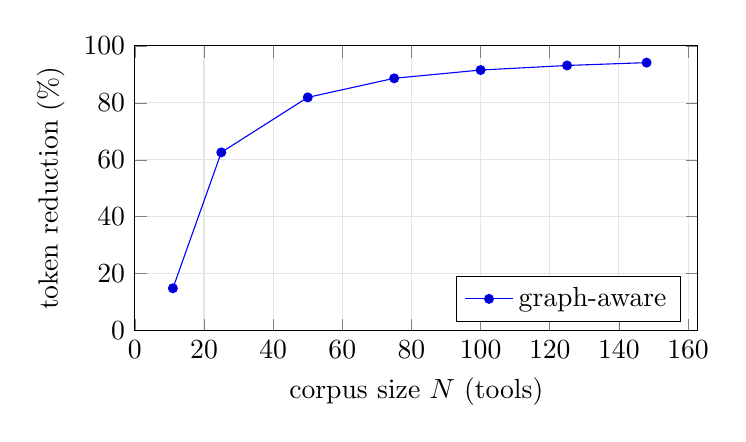
\begin{tikzpicture}
\begin{axis}[
  width=0.72\linewidth, height=5.2cm,
  xlabel={corpus size $N$ (tools)}, ylabel={token reduction (\%)},
  xmin=0, ymin=0, ymax=100, grid=both, grid style={black!10},
  legend pos=south east, mark size=1.6pt,
]
% AUTO-GENERATED by paper/make_results.py
\addplot coordinates {(11,14.9) (25,62.6) (50,81.9) (75,88.6) (100,91.5) (125,93.1) (148,94.1)};

\legend{graph-aware}
\end{axis}
\end{tikzpicture}
\caption{Per-query tool-schema token reduction vs.\ corpus size.}
\label{fig:reduction}
\end{figure}

\begin{figure}[h]
\centering
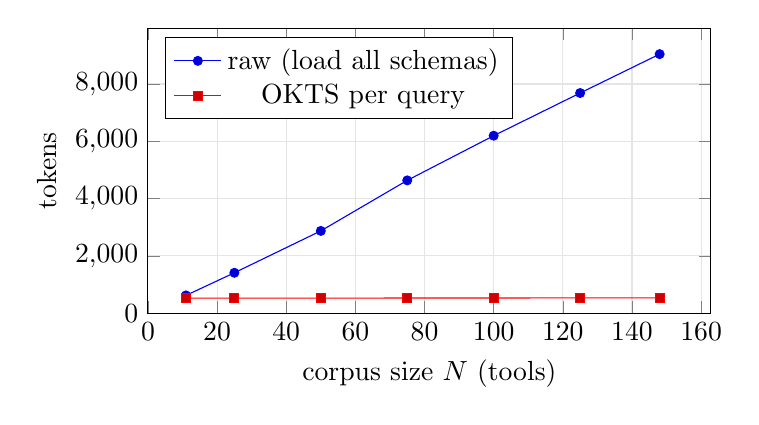
\begin{tikzpicture}
\begin{axis}[
  width=0.72\linewidth, height=5.2cm,
  xlabel={corpus size $N$ (tools)}, ylabel={tokens},
  xmin=0, ymin=0, grid=both, grid style={black!10},
  legend pos=north west, mark size=1.6pt,
]
\addplot coordinates {(11,618) (25,1408) (50,2870) (75,4634) (100,6193) (125,7683) (148,9041)};

\addplot coordinates {(11,526) (25,526) (50,521) (75,528) (100,529) (125,531) (148,531)};

\legend{raw (load all schemas), OKTS per query}
\end{axis}
\end{tikzpicture}
\caption{Absolute token cost: the load-everything baseline grows linearly; the
OKTS per-query cost stays near-constant.}
\label{fig:tokens}
\end{figure}

% =============================================================================
\section{The Infrastructure Comparison}
\label{sec:infra}
% =============================================================================

The quantitative evaluation above compares against a strong \emph{lexical}
baseline. The more consequential comparison for practice is architectural, against
embedding-RAG tool search. Table~\ref{tab:infra} summarizes the asymmetry. OKTS
attains near-ceiling selection accuracy and \reductionFull\% token reduction while
requiring \emph{no} embedding model, \emph{no} inference API in the query path,
\emph{no} vector store, and \emph{no} re-embedding when a tool changes---the index
is portable text, and an edit re-ranks immediately. A learned embedder can be
injected for a possible further lift, but doing so reintroduces precisely these
costs; we regard the zero-infrastructure configuration as the default and the
learned embedder as an optional upgrade, and we benchmark the former. The table
compares \emph{standing operational requirements}, which are architectural facts,
not measured quantities; we make no claim about relative ranking quality here
(see \S\ref{sec:limits}).

\begin{table}[h]
\centering
\caption{Architectural comparison. OKTS keeps retrieval's benefit without the
standing infrastructure of embedding-RAG.}
\label{tab:infra}
\small
\begin{tabular}{lll}
\toprule
Dimension & Embedding-RAG tool search & OKTS (default) \\
\midrule
Index artifact        & opaque float vectors      & portable OKT Markdown (git-diffable) \\
Add / edit a tool     & re-embed (model / API)    & edit text; re-rank immediately \\
Query-path dependency & embedding model reachable & none (lexical + hashing) \\
Vector store          & required                  & none \\
Explainability        & cosine score              & edge provenance + inspectable text \\
\bottomrule
\end{tabular}
\end{table}

% =============================================================================
\section{Limitations and Threats to Validity}
\label{sec:limits}
% =============================================================================

\paragraph{Retrieval-level, not end-to-end.} We measure whether search ranks the
correct tool, not whether an LLM completes the downstream task better. End-to-end
agent success is left to future work (it requires an agent loop and API budget).

\paragraph{Hand-authored corpus and mechanical retrieval text.} The
\numServers{} tool lists are realistic approximations of published surfaces, not
live captures; exact tool counts and parameters will differ by server version.
The bodies are produced by the deterministic offline enricher rather than written
by hand or by an LLM, so the retrieval prose is thinner than a production bundle's
would be. The adapter path is identical for live captures, but absolute numbers
should be read as indicative.

\paragraph{Small, author-labeled query set.} With \numQueries{} queries near a
\graphAccOne\% ceiling, a single query is worth $2.4$ points of accuracy@1;
the full retriever's margin over the baseline is two queries, and its perfect
collision-avoidance score rests on two. Effect sizes are small, we report no
significance tests, and the labels are our own. A larger, independently labeled
set would sharpen the accuracy claims.

\paragraph{Structural signals are unvalidated at scale.} The ablation shows the
hierarchy prefilter and graph expansion to be accuracy-neutral here, and we
attribute that to a corpus whose derived categories are mostly singletons. That
is an explanation, not evidence: we have not tested a corpus where the hierarchy
is coarse enough for the prefilter to discriminate, so the case for these signals
rests on the fixed result count and on surfacing alternatives, both of which are
mechanical properties rather than measured wins.

\paragraph{No live embedding-RAG baseline.} We compare to BM25 quantitatively and
to embedding-RAG only architecturally (\S\ref{sec:infra}); we do not claim to beat
a tuned semantic retriever on ranking quality---only to match a strong lexical
baseline and reach high absolute accuracy without its infrastructure.

% =============================================================================
\section{Conclusion}
% =============================================================================

OKTS shows that an LLM agent can be given a large, multi-source tool catalog while
seeing only three tools, paying a near-constant token cost (a \reductionFull\%
reduction at \numTools{} tools), and selecting the right tool with high accuracy
using a fully offline, zero-infrastructure retriever. The tool's durable unit is a
portable, reviewable descriptor rather than an opaque vector, and the ranking
gain over a strong lexical baseline comes for free from a deterministic hashing
signal---no embedding model, API, or vector store to maintain. We report our
ablation honestly, including that the category hierarchy and graph expansion are
accuracy-neutral on this corpus and instead serve to fix the returned-result count
and surface alternatives. We hope the OKT descriptor and the accompanying open
harness make multi-source tool serving easier to build, evaluate, and trust.

% =============================================================================
\appendix
\section{Reproducibility}
\label{sec:repro}
% =============================================================================

Every number in this paper is produced by \texttt{paper/make\_results.py}, which
builds the corpus and runs the same \texttt{okts.eval} harness the test suite
uses, then writes the tables and plot data this document \texttt{\textbackslash
input}s. To reproduce:

\begin{lstlisting}[style=okt]
pip install -e ".[serve,dense]" tiktoken
python -m okts.eval.corpus --k 5     # headline compare + reduction sweep
python paper/make_results.py         # regenerate all tables/figures
\end{lstlisting}

The \texttt{dense} extra installs \texttt{numpy}, which the hybrid retriever
requires; \texttt{tiktoken} is optional but without it token counts fall back to
the \texttt{chars/4} heuristic and will not match the figures reported here. The
corpus lives in \texttt{eval/corpus/} and the labeled queries in
\texttt{eval/corpus\_queries.yaml}. Every quantity in the running text---corpus
and query-set statistics, retriever hyperparameters, and each ablation row cited
by name---is emitted as a \LaTeX{} macro by the same script, so no number in this
paper is typed by hand. Token counts use \tokenizerName. Code:
\url{https://github.com/prabhukirangit/OKTS}.

\bibliographystyle{plainnat}
\bibliography{refs}

\end{document}
